\documentclass{article}
\usepackage[utf8]{inputenc}

\title{Part 1 - Author Interest Diversity}
\author{Ella Guest}
\date{February 2019}

\usepackage{natbib}
\usepackage{graphicx}
\usepackage{booktabs}
\usepackage{xcolor}
\usepackage{caption}
\usepackage{subcaption}
\usepackage{amsmath}


\begin{document}

\maketitle

\tableofcontents

\listoffigures
 
\listoftables

\section{Methodology Overview}
\begin{itemize}
    \item understand how subreddit communities vary in the extent to which they engage with a diverse range of subreddits
    \item most measures in this section are performed at the author-level, and then aggregated by subreddit
\end{itemize}


\subsection{How does interest diversity vary between subreddits }
For each author I will calculate the number of subreddits they commented in and b) the comment entropy. The subreddit count will give a general idea of author activity on Reddit. The comment entropy will give a better understanding of how equally authors divide their contributions across the subreddits they frequent.


\subsection{How do ‘chamber’ members concentrate within the chamber?}

The literature on echo chamber suggests that confirmation bias encourages people to enter and maintain echo chambers, as we experience pleasure from having our opinions re-affirmed by a group. To test this hypothesis I will determine whether authors who choose to comment in the case study echo chamber spend relatively more time within the chamber than authors in other subreddits. This research question has two sub questions.

\subsubsection{Do chamber members spend more time within the chamber than members of other communities?}

To test this I will measure the in-subreddit ratio for each author, for each subreddit they comment in. The in-subreddit ratio is the number of comments made within the subreddit as a fraction of the total number of comments the author made.

\subsubsection{How does author activity vary within subreddits}

The literature suggests that the majority of participation in online communities is heavily unequal. I seek to determine whether this phenomenon hold for echo chambers. I suggest two two possible scenarios: a) chambers are more unequal as they have a more active core of devoted members, or, conversely b) they are more equal as their members are generally equally devoted. I do not yet have a working hypothesis based on the literature on which direction echo chamber participation should be theorised to lean, though my intuition is A.

To measure participation inequality I will first use the same entropy measure from 1.1. This subreddit author entropy will look at the range in number of comments made by all authors. I will then use a more traditional measure of participation inequality, though I have not yet determined which. Options include the gini coefficient and the Pareto principle but I need to do a small literature review to determine which measure has been most appropriately and successfully used for online communities.


\subsection{Diversity Measures}
For each subreddit $y_i$ there are $n$ comment authors. For the $nth$ author in subreddit $y_i$ there are $x_n$ number of comments, such that for each subreddit we have the vector:

$$y_i = [x_1, x_2, \cdots x_n]$$

I then use this vector to calculate each of the diversity measures (entropy, blau, gini).


\subsubsection{Entropy}

"Information entropy is the average rate at which information is produced by a stochastic source of data." The lower the probability of a value, the greater the "information" it carries. The higher the entropy, the greater the disorder or uncertainty.

Within the context of subreddits, if an author only makes a few comments in the subreddit, any new content they bring to subreddit provides relatively more information... Therefore the higher a subreddit's entropy the greater the diversity...


$$Entropy = -\sum p_ilog(p_i)$$

where $p_i$ is the probability of value $x_i$;

$$p_i = \frac{x_i}{\sum x}$$

The maximum entropy for a subreddit is $log(n)$ thus be can normalise entropy as:

$$Entropy_{norm} = \frac{Entropy}{log(n)}$$

\subsubsection{Blau index}

The Blau index is also known as the Gini-Simpson index, or the Gibbs-Martin index. The Blau index of diversity has a range of 0 to 1, where 0 means the population of perfectly homogeneous, and 1 means the population if perfectly heterogeneous. Therefore the higher the a subreddit's blau, the more heterogeneous the distribution of comments amongst authors, the greater the diversity.


\textcolor{red}{Need to look into using 'true diversity' - it's much more informative for more active subreddits (and more correlated to entropy). Can the "effective number of types" show a diversity threshold?}

$$Blau = 1 - \sum (\frac{x_i}{\sum x_n})^{2}$$

\subsubsection{Gini coefficient}

The gini coefficient is a measure of inequality in a distribution. It is a ratio between the values of 0 and 1, where 0 means perfect equality and 1 means perfect inequality. Therefore the higher the value of gini for a given subreddit, the more unequally comments are distributed across authors within the subreddit.

$$Gini = \frac{1}{n}(n+1-2\frac{\sum(n+1-i)y_i}{\sum y_i})$$

\subsubsection{Justifications of Measures}

Citations for equations and precedence?


\section{Analysis}

The example findings are from February 2018, until I re-run the rest of 2018. In February 2018 86,467,179 comments were made across 104,042 subreddits by X authors. \textcolor{red}{This is calculated post-deleted, when settle on date get pre-deleted vs post-deleted counts.}

\subsection{General Trends}

Table \ref{subLevelDesc} shows that at least half of subreddits had 3 or fewer unique comment authors in February 2018, and 4 or fewer comments. For both count measures the upper quartile is still smaller that the maximum values. I therefore decided to subset the top decile of subreddits by author count as active communities.


\subsection{Default Subreddits}
50 subreddits were at one time classified as a default. Any new redditor was automatically subscribed to the default subreddits. Reddit used default subreddits until May 2017, but those subreddits appear to still benefit in size from their former visibility.

Figures \ref{hist:author} and  \ref{hist:comment} and well as Table \ref{subLevelDesc} show that authors and comments are very unevenly distributed on Reddit, with the majority of subreddits having fewer than 13 and 26 authors and comments. respectively in the February 2018.

Of the 20 subreddits with more than 60,000 authors 14 are default subreddits. However, of the 16 subreddits with more than 500,000 comments only 7 are defaults. In order to run the analysis, I was to remove inactive subreddits from the sample. Given the substantial difference between the most highly active, subreddits on the top end, and the low upper quartile values, I decide to subset the top decile of subreddits by author count. The analysed subset therefore consists of 10,404 of the original 104,042 subreddits.


\subsubsection{Understanding Diversity Mechanics}

Can we examine the defaults to understand the relationship between size, author breakdown and diversity?



\subsection{Subsetting Active Subreddits}
Table \ref{table:all} shows that at least half of subreddits had 3 or fewer unique comment authors in February 2018, and 4 or fewer comments. For both count measures the upper quartile is still smaller that the maximum values. I therefore decided to subset the top decile of subreddits by author count as active communities.

Either one or both of \textit{author count} and \textit{comment count} can be used as a proxy for subreddit activity. In the full dataset the counts have a very strong positive correlation (coef = 0.899). 

As shown in table \ref{table:active}, the lower quartile for blau is 0.98. 90\% of the subsetted subreddits have a value of blau greater than or equal to 0.96.  This, blau does not appear to be an informative measure for active subreddits



% Tables

\begin{table}
\centering
\begin{tabular}{lrrrrr}
\toprule
{} &  log10\_author\_count &  log10\_comment\_count &  entropy\_norm &  gini &  blau \\
\midrule
mean &               0.854 &                1.072 &         0.915 & 0.196 & 0.572 \\
std  &               0.874 &                1.045 &         0.106 & 0.216 & 0.380 \\
min  &               0.000 &                0.000 &         0.003 & 0.000 & 0.000 \\
25\%  &               0.000 &                0.301 &         0.885 & 0.000 & 0.000 \\
50\%  &               0.602 &                0.778 &         0.939 & 0.150 & 0.684 \\
75\%  &               1.322 &                1.643 &         0.985 & 0.352 & 0.916 \\
max  &               5.835 &                6.689 &         1.000 & 0.982 & 0.999 \\
\bottomrule
\end{tabular}

\caption{Descriptive Statistics for all Subreddits}
\label{table:all} 
\end{table}


\begin{table}
\centering
\begin{tabular}{lrrrrr}
\toprule
{} &  log10\_author\_count &  log10\_comment\_count &  entropy\_norm &  gini &  blau \\
\midrule
mean &               4.494 &                4.945 &         0.827 & 0.556 & 0.965 \\
std  &               0.612 &                0.656 &         0.111 & 0.110 & 0.063 \\
min  &               2.248 &                2.702 &         0.394 & 0.269 & 0.678 \\
25\%  &               4.238 &                4.630 &         0.791 & 0.480 & 0.969 \\
50\%  &               4.492 &                4.957 &         0.876 & 0.554 & 0.990 \\
75\%  &               4.937 &                5.340 &         0.896 & 0.619 & 0.994 \\
max  &               5.835 &                6.689 &         0.931 & 0.833 & 0.997 \\
\bottomrule
\end{tabular}

\caption{Descriptive Statistics for Default Subreddits}
\label{table:defaults} 
\end{table}


\begin{table}
\centering
\begin{tabular}{lrrrrr}
\toprule
{} &  log10\_author\_count &  log10\_comment\_count &  entropy\_norm &  gini &  blau \\
\midrule
mean &               2.776 &                3.311 &         0.873 & 0.542 & 0.983 \\
std  &               0.528 &                0.642 &         0.065 & 0.131 & 0.036 \\
min  &               2.134 &                2.155 &         0.061 & 0.000 & 0.078 \\
25\%  &               2.354 &                2.808 &         0.846 & 0.453 & 0.982 \\
50\%  &               2.647 &                3.183 &         0.883 & 0.545 & 0.989 \\
75\%  &               3.068 &                3.707 &         0.914 & 0.637 & 0.993 \\
max  &               5.835 &                6.689 &         1.000 & 0.979 & 0.999 \\
\bottomrule
\end{tabular}

\caption{Descriptive Statistics for Top Decile of Subreddits by Author Count}
\label{table:active} 
\end{table}



% Figures

\begin{figure}
     \centering
     \begin{subfigure}[b]{0.49\textwidth}
         \centering
         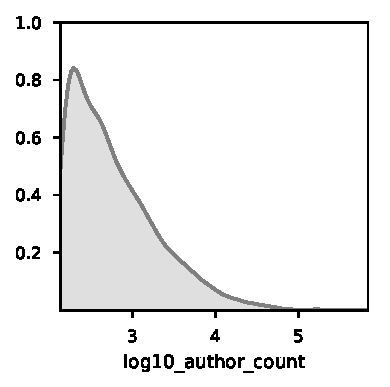
\includegraphics[width=\textwidth]{kde-log10_author_count.pdf}
         \label{hist:author}
     \end{subfigure}
     \hfill
     \begin{subfigure}[b]{0.49\textwidth}
         \centering
         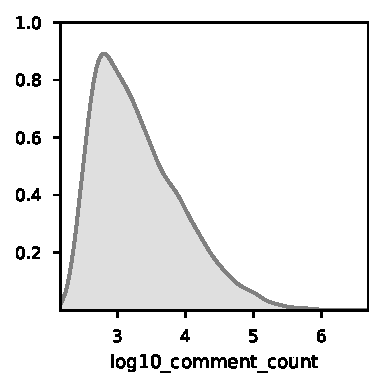
\includegraphics[width=\textwidth]{kde-log10_comment_count.pdf}
         \label{hist:comment}
     \end{subfigure}
     \hfill
     \begin{subfigure}[b]{0.49\textwidth}
         \centering
         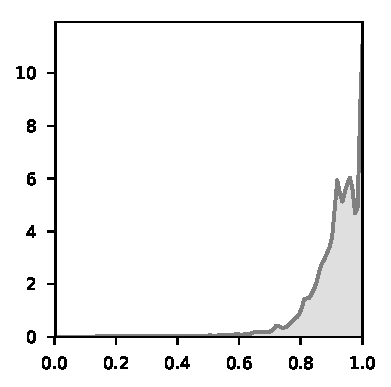
\includegraphics[width=\textwidth]{kde-entropy_norm.pdf}
         \label{hist:entropy}
     \end{subfigure}
     \hfill
     \begin{subfigure}[b]{0.49\textwidth}
         \centering
         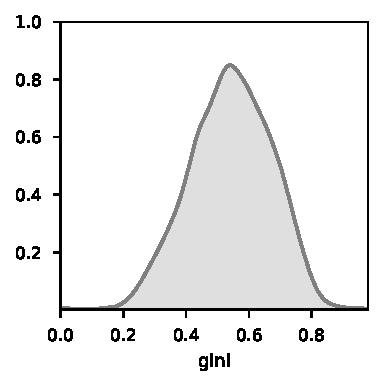
\includegraphics[width=\textwidth]{kde-gini.pdf}
         \label{hist:gini}
     \end{subfigure}
        \caption{Distributions of Active Subreddit Statistics}
        \label{hists}
\end{figure}



\section{Robustness Checks}

\subsection{Longitudinal Variation}

Show stability of variable over time

\subsection{Subsetting by Comment Count}

Re-run analysis on another month


\end{document}
